\documentclass[letter]{article}

%% Language and font encodings
\usepackage[english]{babel}
\usepackage[utf8x]{inputenc}
\usepackage[T1]{fontenc}
\usepackage{enumitem}
\usepackage{fancyhdr}
\pagestyle{fancy}

%% Useful packages
\usepackage{amsmath, amsthm, amssymb}
\usepackage{graphicx}
\newtheoremstyle{case}{}{}{}{}{}{:}{ }{}
\theoremstyle{case}
\newtheorem{case}{}


\title{HW Template}
\author{Nicholas Silva Tee}
\lhead{Homework Template}



\begin{document}

\subsection*{Problem 1.17}
\textbf{a. }
\begin{figure}[h!]
	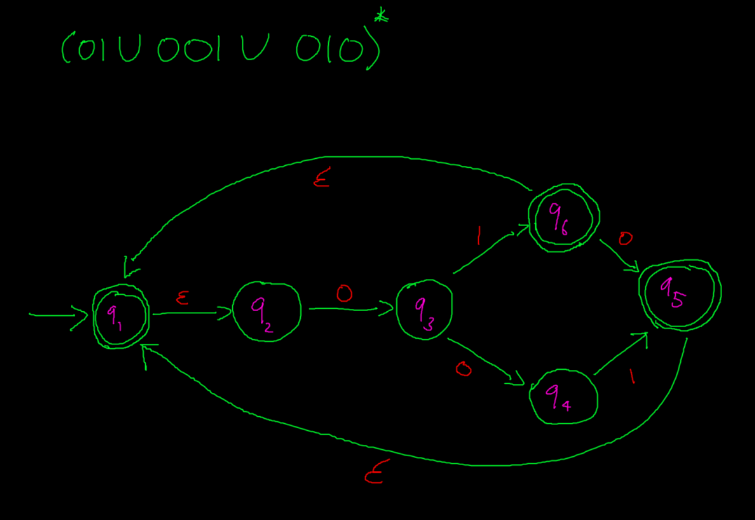
\includegraphics[scale=0.4]{nfa.png}
\end{figure} \\ 

\textbf{b. }
\begin{figure}[h!]
	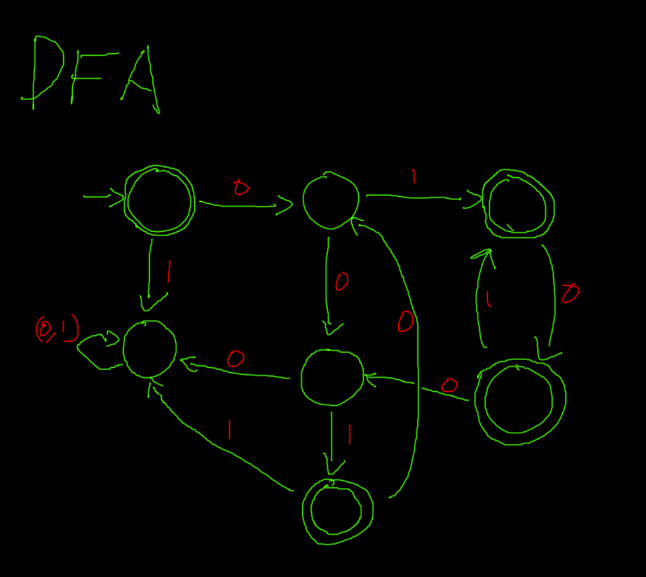
\includegraphics[scale=0.4]{dfa.png}
\end{figure}
\newpage
\subsection*{Problem 1.18}
\textbf{a. } $1\Sigma^*0$\\ 
\textbf{b. } $\Sigma^*1\Sigma^*1\Sigma^*1\Sigma^*$\\ 
\textbf{c. } $\Sigma^*0101\Sigma^*$ \\ 
\textbf{d. } $\Sigma\Sigma0\Sigma^*$ \\ 
\textbf{e. } $0(\Sigma\Sigma)^* \cup (1\Sigma)(\Sigma\Sigma)^*$\\ 
\textbf{f. } $0^*(100^*)*1*$\\ 
\textbf{g. } $(\epsilon \cup \Sigma)^5$\\ 
\textbf{h. } $\epsilon \cup 0\Sigma \cup 10 \cup 10\Sigma \cup 0\Sigma\Sigma \cup 110 \cup \Sigma\Sigma\Sigma\Sigma^* $\\ 
\textbf{i. } $(1\Sigma)^* \cup 1$\\ 
\textbf{j. } $00^* \cup 100^* \cup 010^* \cup 00^*1$\\ 
\textbf{k. } $0 \cup \epsilon$\\ 
\textbf{l. } $0^*10^*10^* \cup 1^*(01^*01^*)^*)$ The 1s and 0s can be shifted around, there are too many cases where there can be even 0s (e.g. 0011111111 which does not apply to the definition) and too many cases of two 1s (e.g. 11000000000) \\ 
\textbf{m. } $\emptyset$\\ 
\textbf{n. } $\Sigma^*$\\ 
\subsection*{Problem 1.19}
\textbf{a. }
\begin{figure}[h!]
	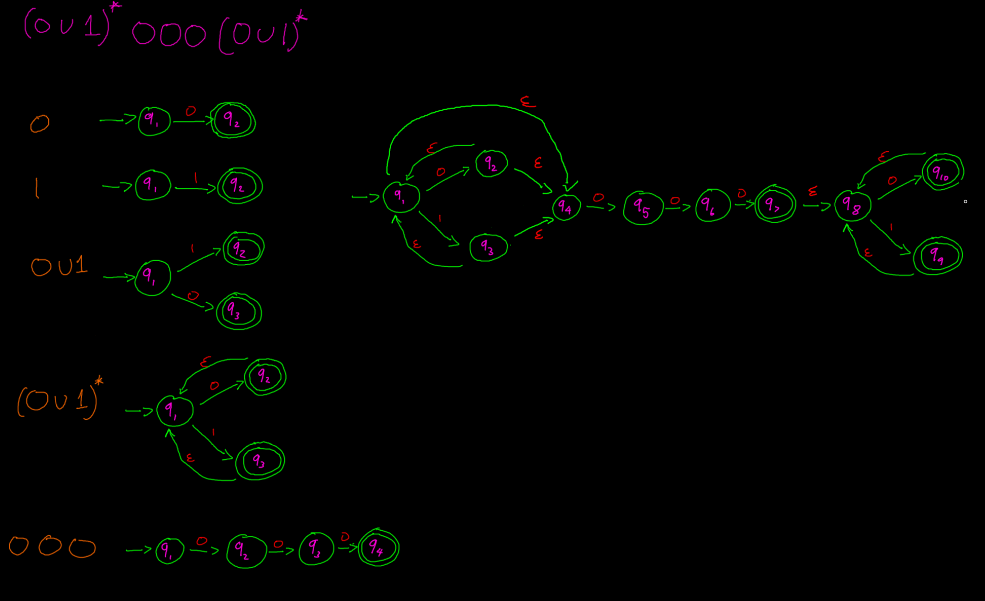
\includegraphics[scale=0.4]{19a.png}
\end{figure}
\newpage
\textbf{b.}
\begin{figure}[h!]
	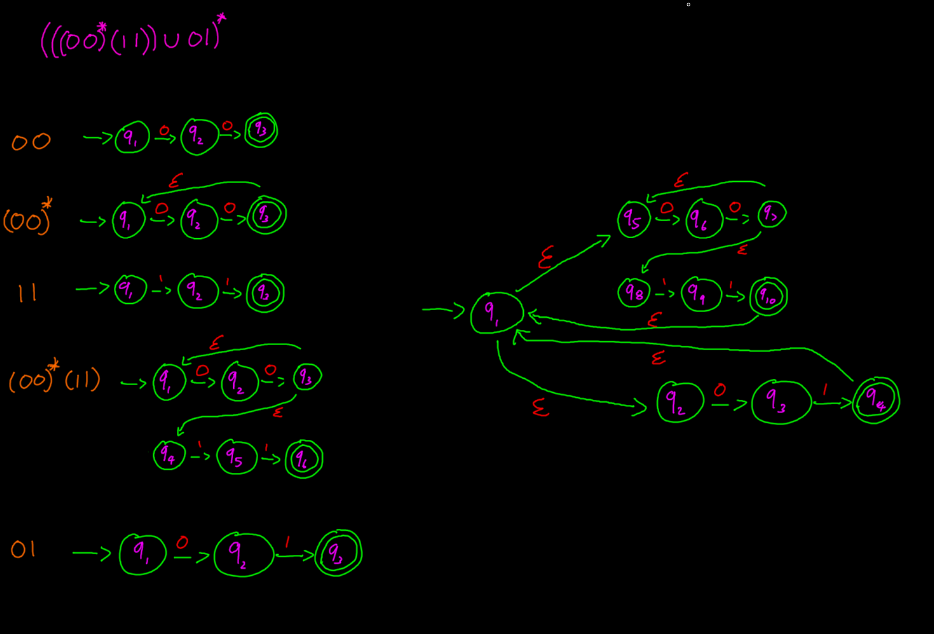
\includegraphics[scale=0.4]{19b.png}
\end{figure} \\  
\textbf{c. }
\begin{figure}[h!]
	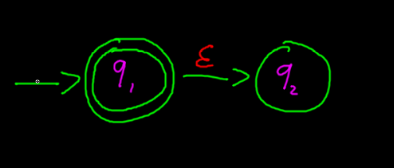
\includegraphics[scale=0.4]{19c.png}
\end{figure}
\end{document}










